% The intervals of length at most p_max that contain a time step t.
% Adapted from the slide "Data Reduction Procedure" and Figure 4 of the paper.
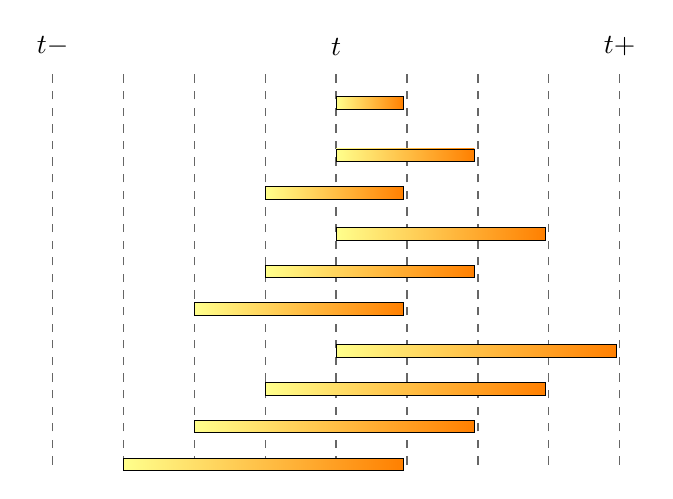
\begin{tikzpicture}[scale=0.9]
\def\dy{3}
\def\barh{0.09}
\foreach \x in {-4,...,4}
    \draw[line width=0.5pt, dashed, opacity=0.6] (\x,-5.3) -- (\x,0.25);
\node at (-4,0.6) {$t-\pmax$};
\node at (0,0.6) {$t$};
\node at (4,0.6) {$t+\pmax$};
\foreach \i/\p in {1/1,2/2,3/3,4/4}
{
    \pgfmathtruncatemacro{\pstar}{\p - 1}
    \foreach \r in {-\pstar,...,0}
    {
        \pgfmathsetmacro{\y}{\r/\dy - \i*.85*\i/\dy + \i/\dy+\r*.2+.25/(\i*\i*\i)-.5}
        \pgfmathsetmacro{\xend}{\r+\p-0.05}
        \shade[left color=yellow!45, right color=orange] (\r,\y-\barh) rectangle (\xend,\y+\barh);
        \draw[line width=0.35pt] (\r,\y-\barh) rectangle (\xend,\y+\barh);
    }
}
\end{tikzpicture}
